\begin{abstract}
 The abstract goes here...
\end{abstract}




%*****************************************
\chapter{Introduction}
%*****************************************

This chapter gives the background of Serious Game. Which role Serious Game play in city planning and which kind of problems Serious Game concern about today.  

\section{Motivation}
Video games have been in development for decades and are now becoming more and more mature. With an increasing number of categories comes Serious Game, which focuses on specific area comparing with the normal digital games. According to Schmidt et al \cite{schmidt2015applied}, Serious Game can be categorized by the purpose of the game. Following the book of David Michael\cite{michael2005serious}, there are several classifications such as education, governments, healthcare and so on. In addition, some city simulated game have two main charakteristics, 3d models and city mechanisms. The combination of these two can make the game simulate a real city to some extent. It is clearly to be seen that Serious Game may be very helpful in city planning. 

The world we live in is becoming increasingly complex as the social, ecological, economic and infrastructural challenges we face continue to grow. At the same time, the connections and dependencies between individual city management tasks and the impact of their changes are becoming increasingly difficult to assess.

So the logical combination of the vcast amount of information with visible assessment is necessary. Otherwise, the representation of isolated data points that benefit only their respective owners. The ability to quickly and easily assess current information from a central location is more important than ever when it comes to making better decisions on a broader scale.


In the era of Industry 4.0, the word Smart comes more and more popular. The combination of virtual world with reality becomes some new ideas in the development of our city. In 2010, IBM formally put forward the vision of "Smart Planet" \cite{IBMSmartPlanet}, which is seen as the predecessor idea of "Smart City", hoping to contribute to the development of cities in the world. IBM has studied that cities consist of six core systems of different types of networks, infrastructures and environments that relate to the main functions of the city: organization, business, government, transportation, communication, water and energy. The systems are not fragmented, but are interconnected in a collaborative way. The city is a macro system made up of these systems.


\section{Problem Statement and Contribution}
This report focusing on both of the two areas mentioned before, Serious Game and Smart City, trying to discuss how this two areas combined with each other and some technologies can be used. Furthurmore, some applications will also be shown.

\section{Outline}
This article will first focus on the two characteristics of city simulation games mentioned in the previous. Some 3d modelling technologies will be introduced in the 3d modelling chapter. The simulation chpter will talk about how a game simulate the mechanisms of a city, for instance, the water recycle system. after these two main chapter, some applications in Digital Twins and Smart City will be introduced. These two areas These two ideas are very popular today, both in industry and on the Internet area.

%*****************************************
\chapter{3D Modelling techniques}

3D city model represents the city including the urban surrounding based on 3d geometry of city units and a lot of geographical information, for instance, buildings and altitude.  With city building 3D modeling as the carrier, integration of local city buildings, government, enterprises and institutions and other multi-channel resources, information, the most image intuitive electronic map. 3D city models provide many other service functions related to city life, such as searching, positioning,  public transportation inquiry, navigation, sightseeing display, passenger flow display, traffic condition etc.. In conclusion, 3D city model plays a indispensable role in city visualizaion, not only provides convenient living services, but also save the cost of city managment. More and more decision makers are realizing that 3D city models will soon become indispensable central information systems assessible to almost anyone. The high quality of information and reliable spatial visibility they provide and the variety of uses they thus support make these models an invaluable tool for solving a wide range of problems.

Based on the work of Filip Biljecki \cite{biljecki2015applications}, nowadays various 3D modelling techniques can be implemented in producing a city model. This chapter describes achievements of 3D city modelling, and some furthur examples will be mentioned as well. After listing all the techniques, there will be evaluation and comparation in the summary.

\section{photogrammetry and laser scanning}

As Norbert Haala points out \cite{haala2010update}, though automated urban modeling systems still have been a very active field, it is still a intractable problem to generate complex digital building model, since the development of tools for 3D city modeling twenty years ago. Initially, automated city modelling was only for polyhedral building objects, for which photogrammetry and laser scanning were common techniques.   

LiDAR is one of the most widely used techniques in this area. It is an advanced detection method combining laser technology and modern photoelectric detection technique. It consists of transmitting system, receiving system, information processing and other parts. The main idea is: The laser ranger emits a signal to the ground object as a target, and the reflected signal time information received by the receiver is used for distance measurement and detection.This diagram below shows briefly how LiDAR works, more details may be shown in further detail in Zolotaykin's report.

\begin{figure}[htb]
	\centering
	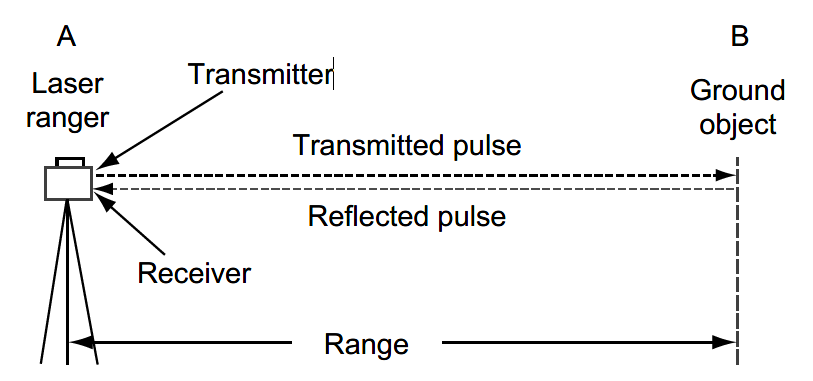
\includegraphics[width=0.7\textwidth]{gfx/LiDAR}  	  	 	
	\caption{How LiDAR works.}
	\label{fig:example1}
\end{figure}



\subsection{Application}

The 3D city model of las vegas in Figure 1 and Figure 2 is based on the automatic generation of high-resolution images.As can be seen in Figure 2, the result is a detailed surface mesh, which can be obtained after the corresponding texture filling of the images in Figure 1.

\begin{figure}[htb]
	\centering	
	\subcaptionbox{The 3D model of Las Vegas 1 %
		\label{fig:example_2}}%
	[.48\linewidth]{
		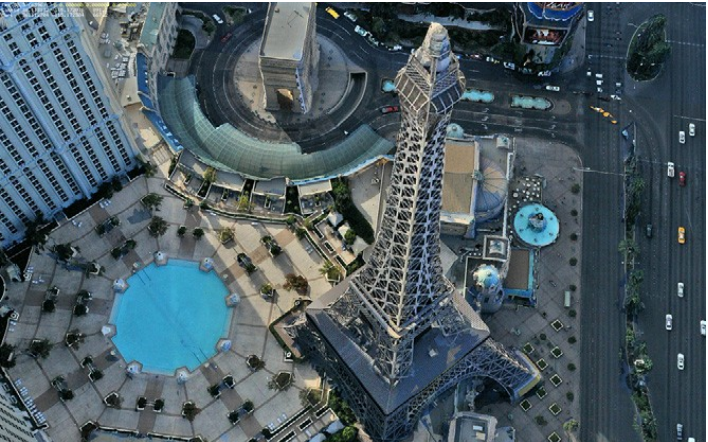
\includegraphics[width=0.45\textwidth]{gfx/LasVegas_1} 	
	}  	
	~
	\subcaptionbox{The 3D model of Las Vegas in mesh view  %
		\label{fig:example_3}}
	[.48\linewidth]{
		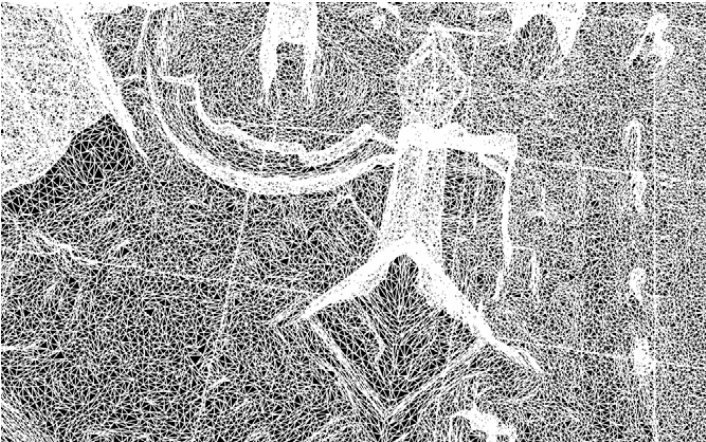
\includegraphics[width=0.45\textwidth]{gfx/LasVegas_2}  	
	}	  
	
	\caption{The 3D model of Las Vegas. \cite{haala2010update}}
	\label{fig:ex_2_3}
\end{figure}

From these two images we can see that at a certain height, the rougher 3d models still have a considerable degree of excellent visualization. However, for higher precision reproduction requirements, even inside buildings, more complex measurement methods and more data points are required.



\subsection{Evaluation}

Nowadays the main applications for interactive visualization of 3D city models are Google earth bing maps, for this kind of large-scale visualization, and the models are usually limited to roof structures and flat facades. In this case, rough and fast automatic modeling is a good approach. Furthurmore, the use of this method is very effective for the reproduction of buildings in rural and suburban areas, as the shape of a large number of buildings is quite simple and repetitive. 

However, it is somewhat weak for high precision building reproduction needs. It is also often restricted to relatively complex landmarks.  the demand for district-based displays is increasing. 

Besides,fully-automatic generated images are hard to comprehensive, sometime it is necessary to involve some semi-automatic components and artificial measurements to support experts for the recognition to the complex building.

Larry Hertz has written a report about the resconstruction of Notro Dame, he mentioned that the digital model of Notre Dame  derived a great help in the reconstruction of it. With more than 50 scans, 5 mm level of accuracy, and 1 billion data points, Andrew Talon created a finely detailed digital model of the church in 2015 by accurately documenting the entirety of Notre Dame's interior and exterior through laser scanning and 3D modeling. Another 3D scanning model of Notre-Dame can be find in the website "Mapping Gothic France" from University Columbia. The open data of Notre-Dame on the website includes floor plans, stereoscopic views, 360° panoramas, laser scanned images, and billion pixel images, allowing visitors to enter Notre-Dame de Paris in all its dimensions through different image formats.

\begin{figure}[htb]
	\centering	
	\subcaptionbox{https://www.youtube.com/watch?v=jAi29udFMKw %
		\label{fig:example_5}}%
	[.48\linewidth]{
		\includegraphics[width=0.45\textwidth]{gfx/Notre_Dame_1} 	
	}  	
	~
	\subcaptionbox{https://mcid.mcah.columbia.edu/art-atlas/mapping-gothic/paris-cath%C3%A9drale-notre-dame  %
		\label{fig:example_6}}
	[.48\linewidth]{
		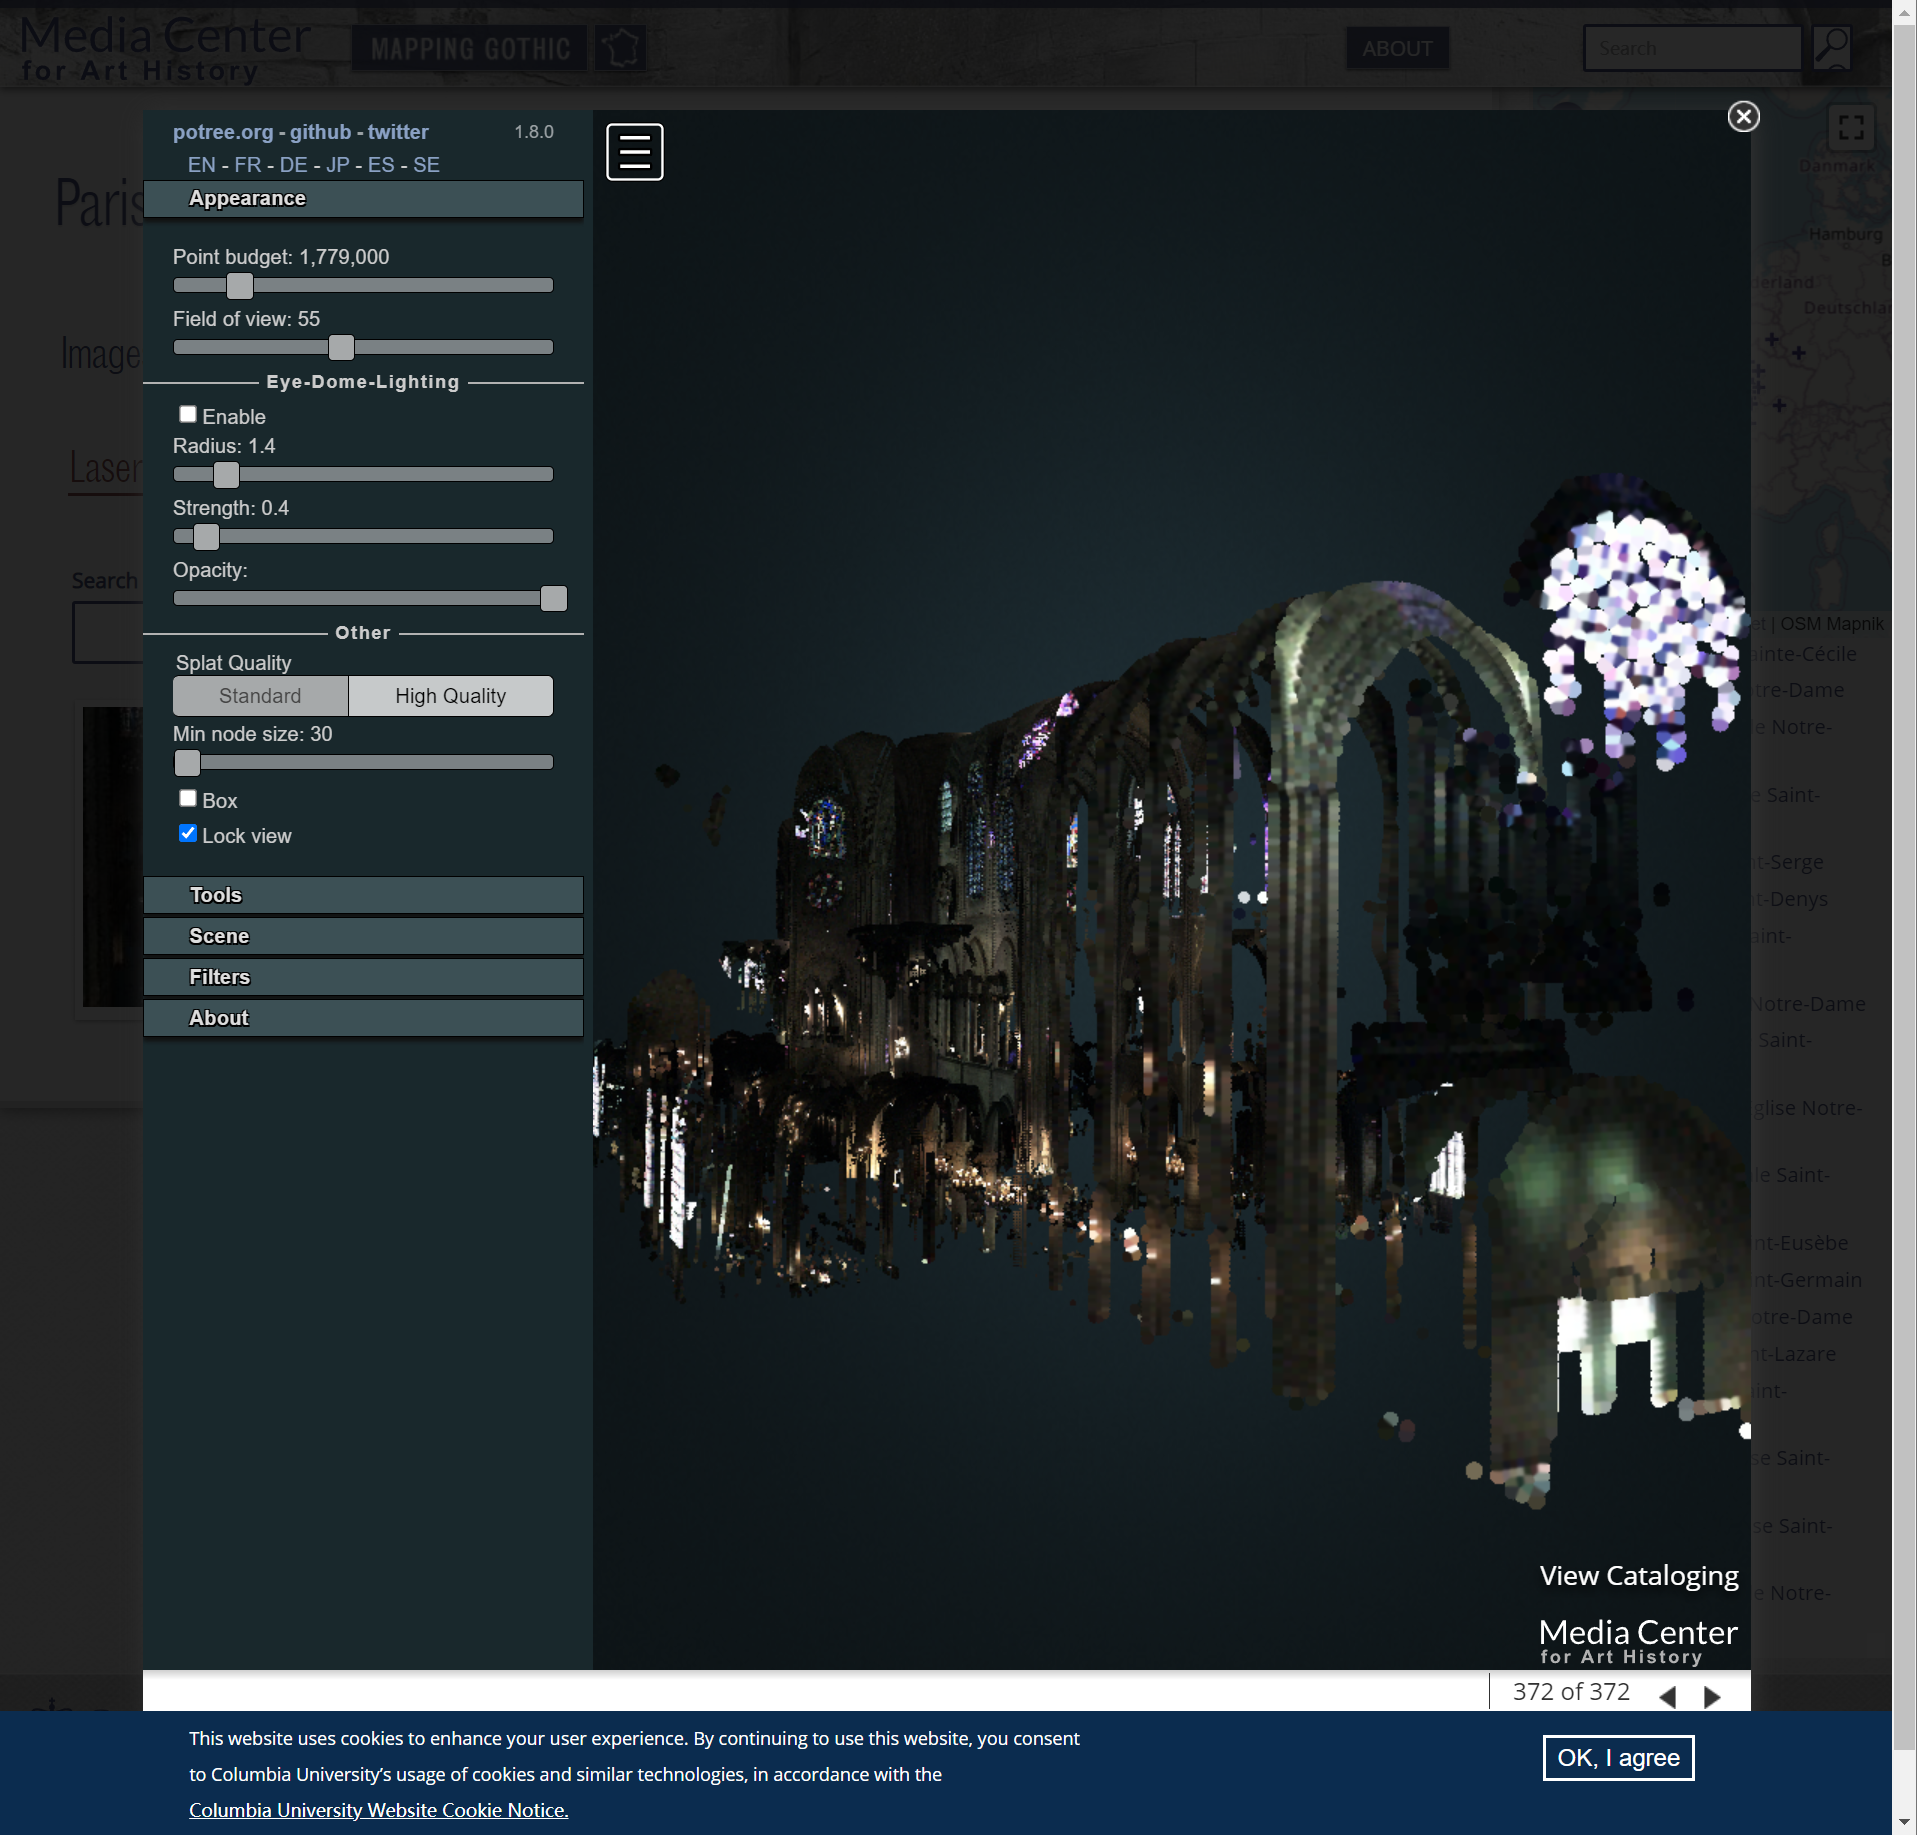
\includegraphics[width=0.45\textwidth]{gfx/Notre_Dame_2}  	
	}	  
	
	\caption{The scan of Notro-Dame.}
	\label{fig:Notro-Dame}
\end{figure}


The other remaining issue can be, different areas such as suburban, rural, commercial and residential areas have different architectural styles, simply showing the exterior model of the building will no longer be a good method, so more detailed geometric reconstructions are necessary. 



\section{Footprint Extraction} 

Therefore, introduction of paramatic building's footprints in the 3D reconstruction process becomes a method, which deals with the region segmentation problem efficiently. 

Fortunately, similar building types are abundant in the reconstruction process. For example, most of the buildings in the countryside are simple and easily generalized by parameters, or specific district of the city have similar roofs over large areas, which can be efficiently identified with low accuracy requirements. This simple method of automatically building a 3d city model using a given set of representative building footprints is called the "extrusion".

\begin{figure}[htb]
	\centering
	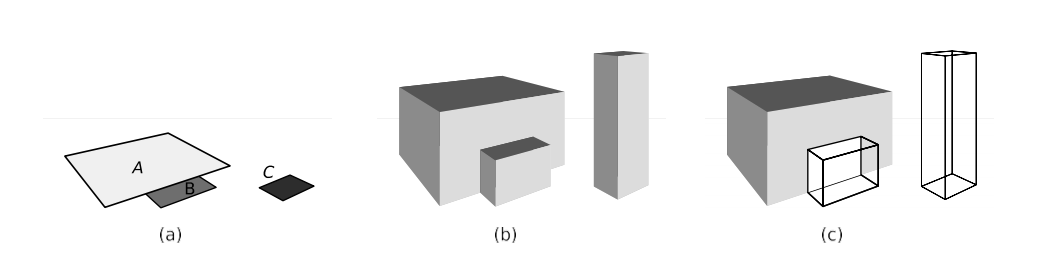
\includegraphics[width=0.7\textwidth]{gfx/extrusion}  	  	 	
	\caption{Extrusion Process.\cite{ledoux2011topologically}}
	\label{fig:extrusion}
\end{figure}

The figure \ref{fig:extrusion} shows the basic process of how to generate 3D model by extrusion. figure(a) is a topograph of a building area, which has three polygons stand for three building components. In the next step, heights are assigned to them, then three polygons are pushed upwards to give figure(b). Thus three polygons are extruded as three polyhedra. In figure(c), based on the topology in figure(a), BC is obtained by the polydedron A.

The extrusion should respect topological consistency, and several several principles: 

1. The polygons suit to the topological footprints. 

2. The roof polygon is the same shape as the door, but all points lie at the same extruded height. 

3. Each line segment becomes a wall, in other words a polygon vertical to the ground.

The benefits of obeying to consistency are: it is easier to maintain consistency as the data set changes over time; also, maintaining consistency allows spatial manipulation of objects and ensures that the results are still valid; in addition, it is easy and simple to use topological data structures to store objects.

However, the extruded 3D building model can not be restored in a topological data structure, which makes the furthur assessment not achievable. The reason is that, the extruded model includes overlapped points and planes, so it does not obey the topological consistency. This issue can be represented in the figure \ref{fig:extrusion}, that the overlap between the separated front faces of building A and B breaks the topological consistency.

Hugo ledoux proposes a simple method\cite{ledoux2011topologically} to extrude the model, and ensure the mapping between 2D topological data and 3D model is consistent.  The input is a 2D topological data set and can be output in a variety of variant data formats. The basic idea of this method is, using constrained trangulation to guarantee the topolocial consistency between the extrusion and terrain.

The specific steps are as follows: Firstly, creating the contrained Delaunay trianglation diagramm as input data set, generating the ground and roof belongs to the specific building by recognizing the triangles in Delaunay trianglation diagramm(Connecting the vertices in the topology diagram and modify it to a graph made entirely of triangles), which are seen as the footprints of the building. Finally, extruding the polyhedron by accessing the constrained edges in Delaunay trianglation diagramm, then a vertical wall of the building is created.

\begin{figure}[htb]
	\centering
	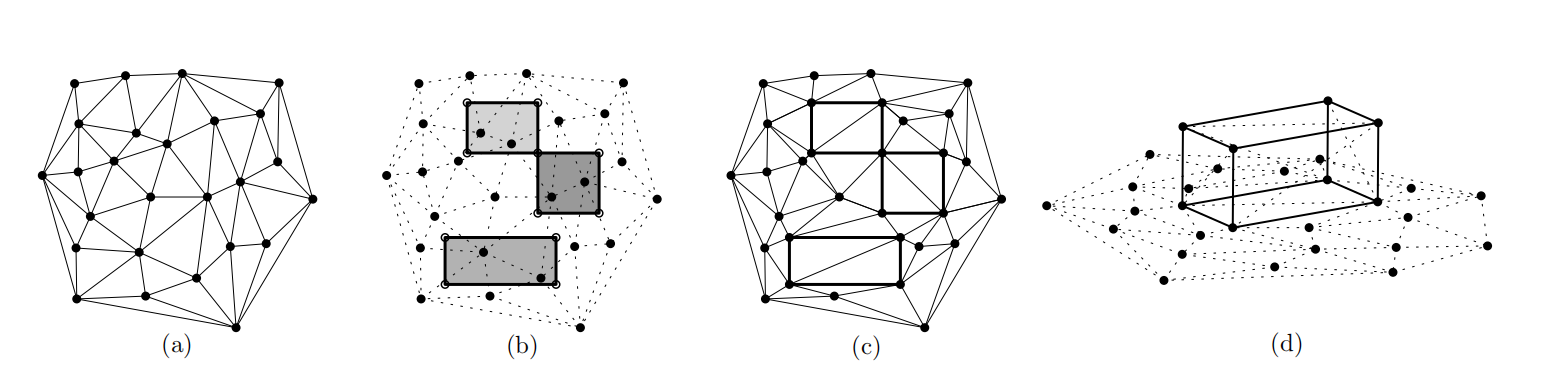
\includegraphics[width=0.7\textwidth]{gfx/triangulation}  	  	 	
	\caption{Triangulation.\cite{ledoux2011topologically}}
	\label{fig:triangulation}
\end{figure}

Figure(a) in \ref{fig:triangulation} is the input constrained Delaunay trianglation diagramm as the terrain. Figure(b) put the topology data with height involved on the terrain. In Figure(c) the three buildings are modified along the constrained Delaunay trianglation diagramm. In figure(d) building adds the height, and is pushed up as an polyhedron.

\subsection{Application}
When we mention a 3d model of any city, people always think of google map. But for many construction co-workers, Google Maps cannot generate working files that can be manipulated directly, some furthur simulation like storm and energy is impossible either. Two 3D city modelling website will be shown in this section, they can achieve the above two needs respectively.

CadMapper(https://cadmapper.com/) is a very convenient 3d map generation website, through which you can get 3d models of any region of the world and apply them to many different softwares such as, AutoCAD, SketchUp etc. CadMapper generates a model based on the city topology map and then adds height data for different buildings. Here is the 3D model generated by CadMapper of Darmstadt city center.

\begin{figure}[htb]
	\centering	
	\subcaptionbox{The 3D model of Darmstadt %
		\label{fig:example_5}}%
	[.48\linewidth]{
		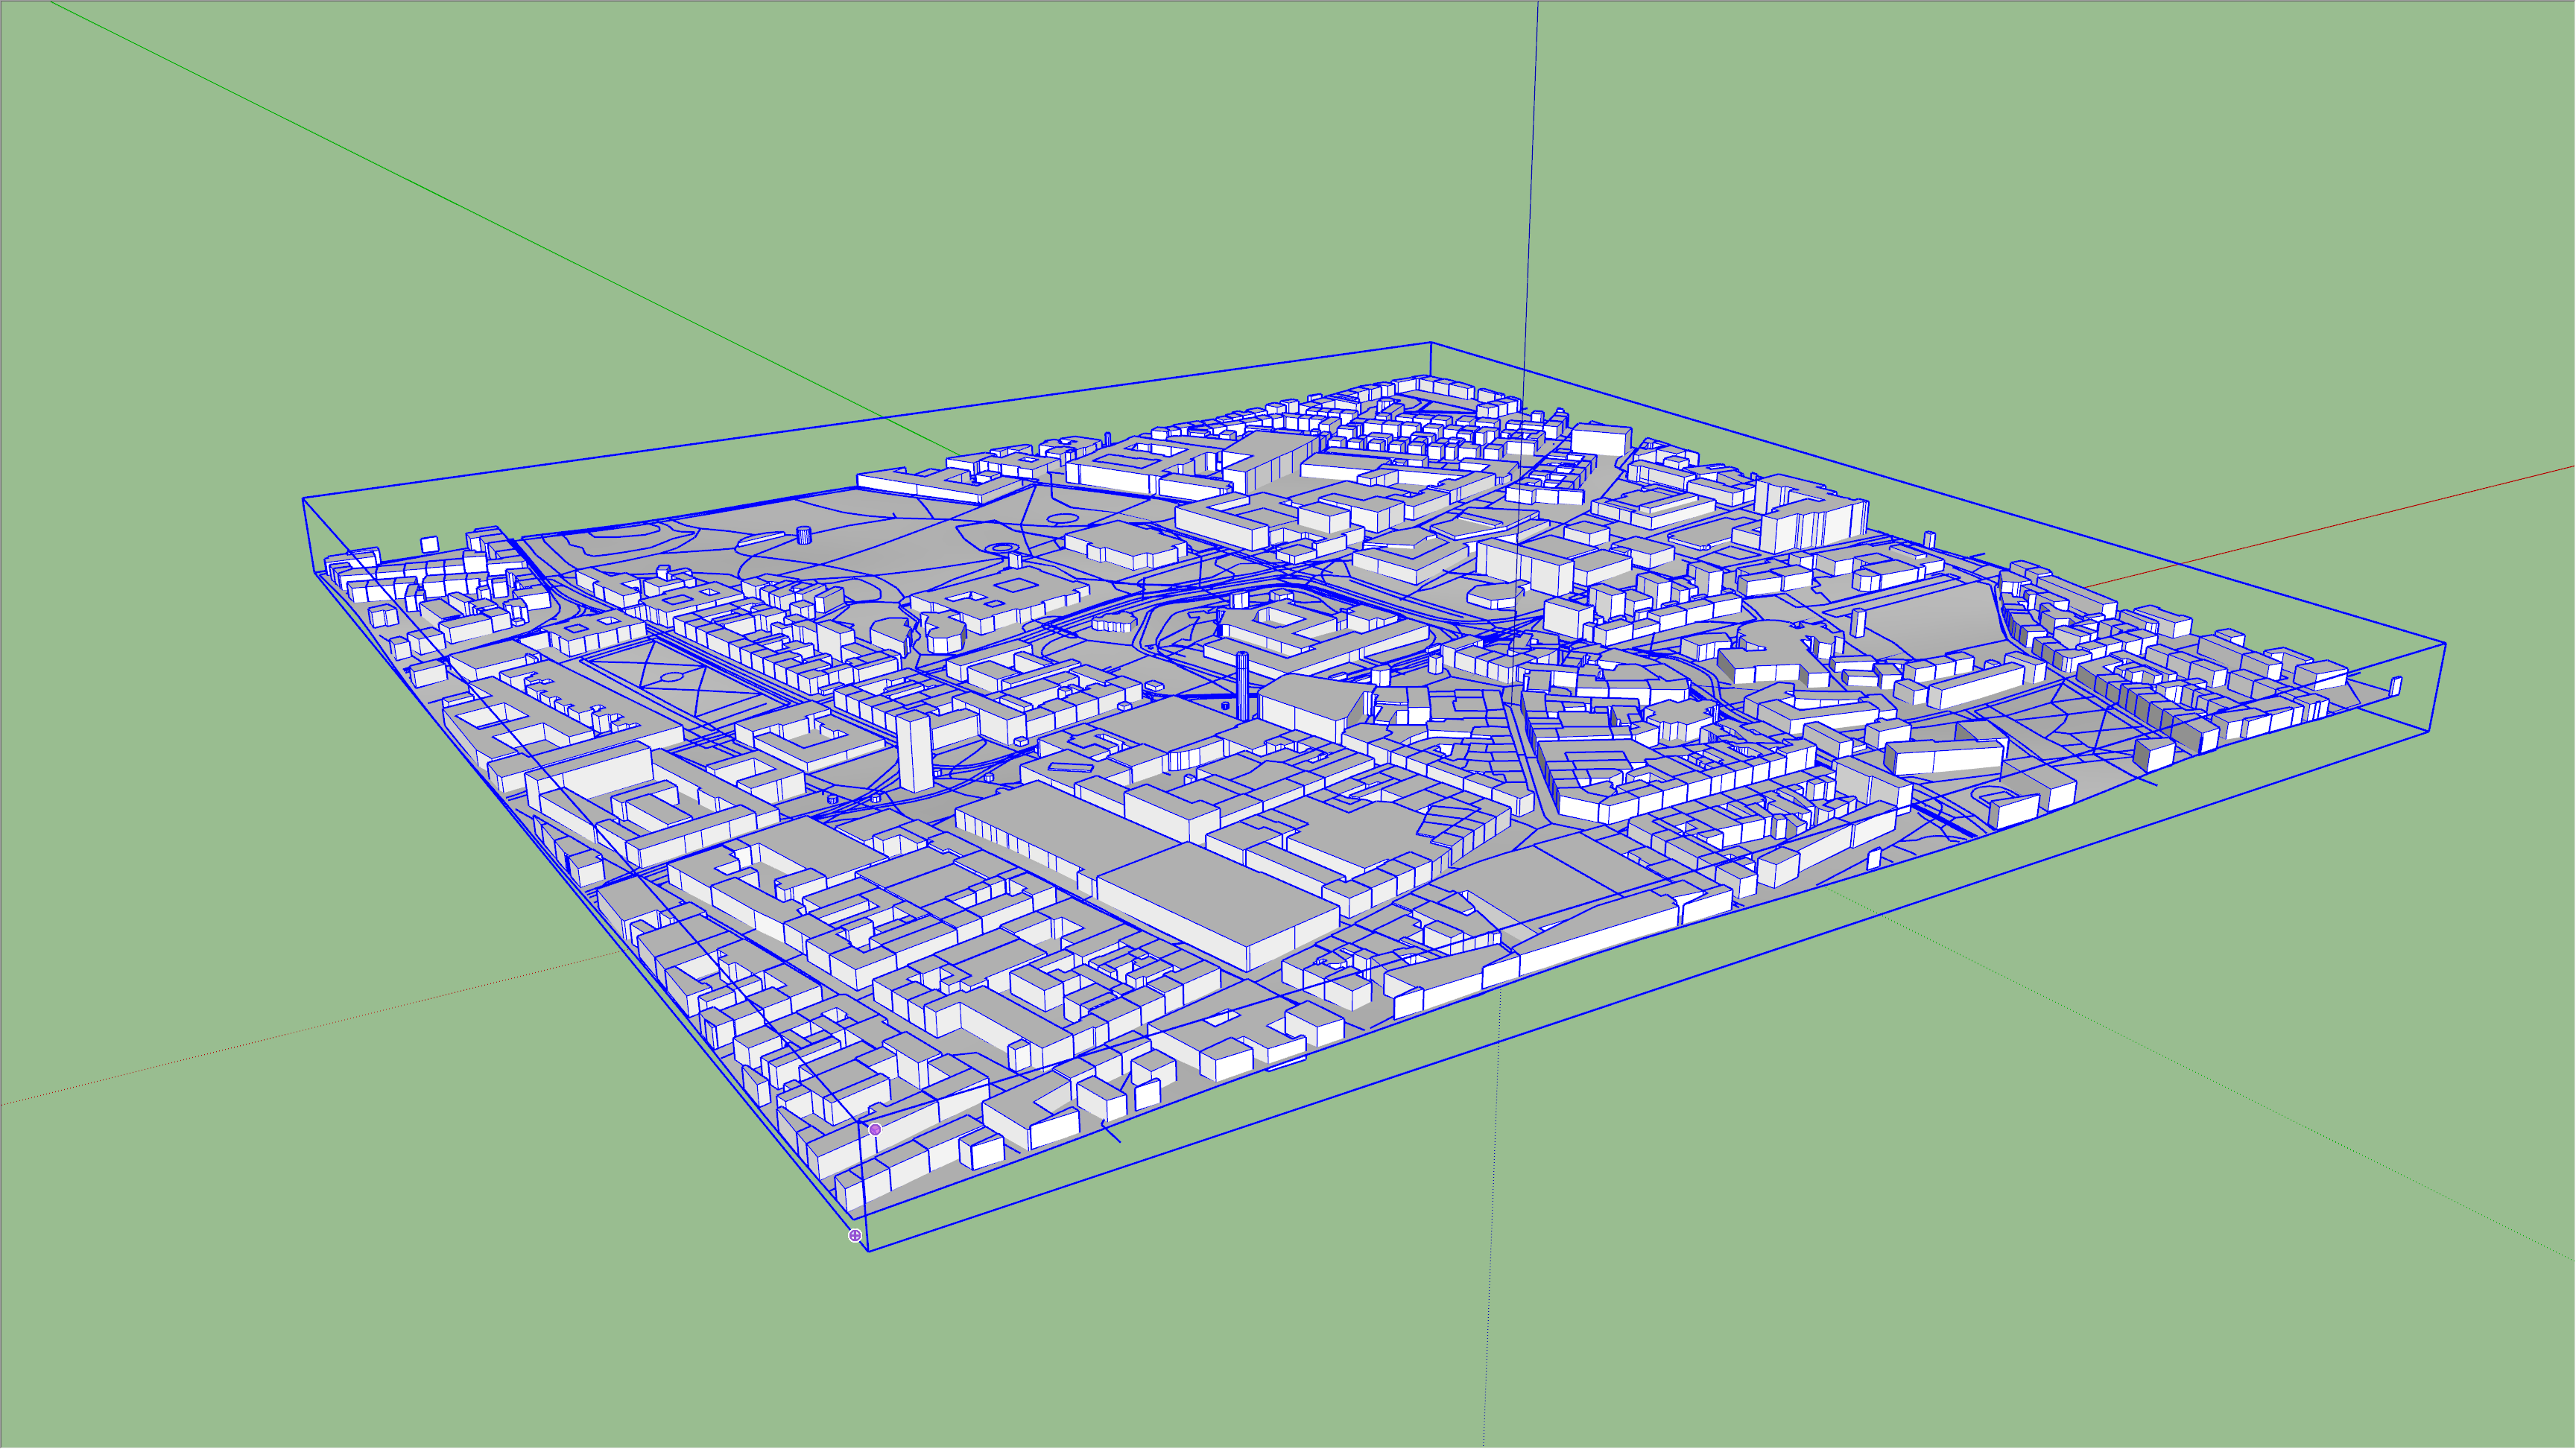
\includegraphics[width=0.45\textwidth]{gfx/Darmstadt} 	
	}  	
	~
	\subcaptionbox{The 3D Axonometric View of Darmstadt  %
		\label{fig:example_6}}
	[.48\linewidth]{
		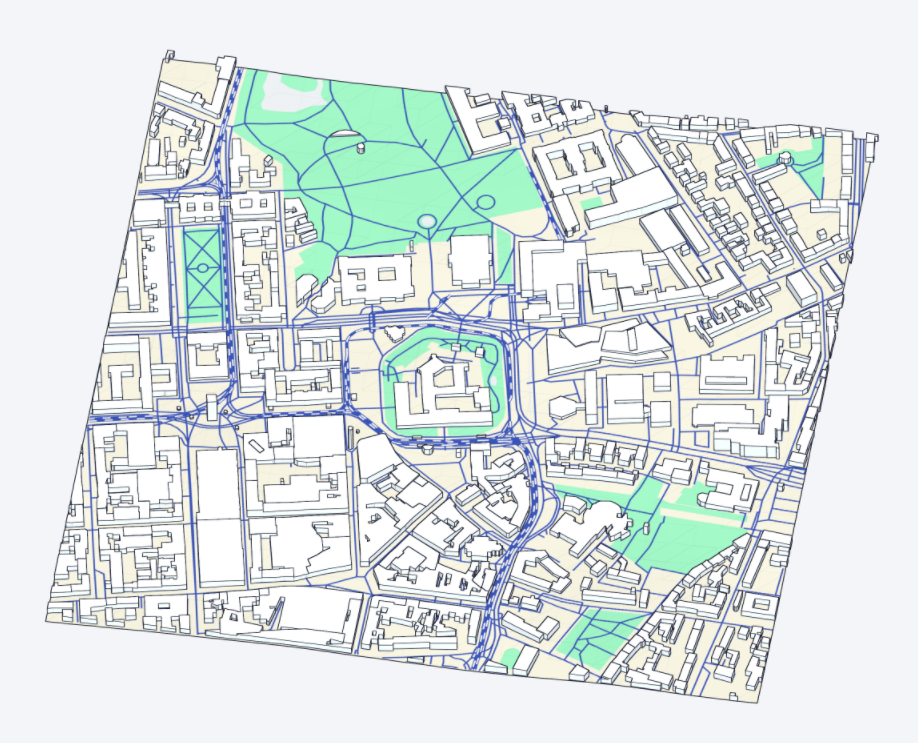
\includegraphics[width=0.45\textwidth]{gfx/Darmstadt_2}  	
	}	  
	
	\caption{Model of Darmstadt in SketchUp 2015.}
	\label{fig:ex_3}
\end{figure}

VirtualCityMap tries to build up a visible information assessment system, based on their 3D city model and, to provide variant solutions such as management, traffic, energy etc.


By providing a way to realistically depict city elements, the 3D city models from VirtualCityMap can display and simulate changes, which can be viewed in advance. In addition to these visualizations, database queries for specific attributes such as height, area can be run directly in the 3D city model.

The functional solution of VirtualCityMap is based on CityGML. It is a format for the exchange and storage of data for virtual 3D city models and is a common datatype for the representation of 3D city templates. It defines the types and interrelationships of the most common surface targets in cities and regions and takes into account the geometric, topological, semantic and appearance properties of the targets, including the hierarchy between thematic types, aggregation, relationships between targets and spatial properties.

\begin{figure}[htb]
	\centering
	\includegraphics[width=0.5\textwidth]{gfx/virtualCityBerlin}  	  	 	
	\caption{The 3D simulated model of Berlin.
		\\https://berlin.virtualcitymap.de}
	\label{fig:berlin}
\end{figure}


\subsection{Evaluation}

Based on the parametric footprints can experts quickly generate a 3d model of a specific area of the city. However, for more precise modeling needs, the basic parametric footprints do not have enough expressive power. The issue is especially significant for buildings with discontinuous heights or asymmetric roofs. Therefore some attempts to segment the building footprint tried to solve this problem.

Kada and McKinley proposes an idea \cite{kada20093d}, decomposing the footprint of most buildings into two parts along the roof. Due to the complexity of the building's footprint and the limitations of the picture's accuracy, precise segmentation, which adapted to the shape of the roof is difficult to achieve. Therefore, spatial partitioning is not generated by decomposing the footprint itself, but by decomposing the enlarged blocks along the approximate linear features of the building and reconstructing them from scratch. The resulting two-dimensional cells are then compared to the original footprints and the parts with low overlap are discarded. The remaining parts then form the approximate shape of the building footprint. This method has been widely used in many urban 3d reconstruction projects.



\section{Synthetic Aperture Radar}

\subsection{Evaluation}

\subsection{Application}

\section{Summary}

%*****************************************
\chapter{Simulation}

In order to finish a geo-based game, not only 3D model is necessary, but also the simulation of the management should be considered, like water system and power system. A realistic simulation makes geo-based game more practical and the educational effect more effective. However different from commertial digital games, the development of serious games is a complex and high cost process that depends on both expertise and software development knowledge. This part of the work may require the involvement of many subject matter experts. 

Heinrich Söbke has mentioned that, due to the interdisciplinary character of serious game, it requires highly cost of development effort. He considered that game engine is a effcient achievement to simplify the process. The rule can be used to integrate more domain-specific features into a game engine or integrated development environment. It could be a supportable tool for learning, education components and serious game with city planning.\cite{sobke2016serious}. In this case, games provide a good visible platform to citizens and decision maker, who may not have professional knowledge, and help them with their decision.

This chapter discuss how geme engine simulates the city as real life. 

\section{GlassBox}

GlassBox is a data-driven simulation engine for Maxis games, which is used in SimCity 2013. It uses agent-based simulation, which is a framework that helps player learn some skills and assess their work with emotional, plausible agents. The concept of agent-based simulation engine make it easier to implement a user friendly interface. The combination of engine with simulation deduces implementation difficulties by replacing programming to a certain extent. With the main paradigm "What you see is what you sim", it simplifies development by the visualization of the simulation process, especially city building games. 

Nonetheless, there is still a problem that, GlassBox is not a open source software, there is also no way for outsiders to implement some of GlassBox's features through the interface. Therefore in this section, it will only be dealed with the introduction of the GlassBox functionality and design logic and the specific implementation methods will not be mentioned.

It was mentioned by Dan Moskowitz in GDC 2012, that GlassBox abeys the priciple "What You See Is What You Simulate.". The previous simulation city game relied on relatively high statistic, the pollution index rose and the happiness index fell. GlassBox is just the opposite. It simulates a few little things, for instance, the behaviour of citizens, so the city mechanics comes naturally. You don't have to look at spreadsheets or graphs to spot crises as you can see all of this in real time. Pollution will pollute the soil and thicken the atmosphere with smog, Sims will get sick and fill hospitals, companies will lose employees, and everyone will get upset about the whole thing. The basics of GlassBox are four aspects: Resources, Units, Maps, Globals.

\subsection{Resources and Units}

Resources can be seen as the currency of the game. There are many difference resources such as coal, water, electricity, oil etc. Units are the basic entities of building, such as house, factory, fire station etc. Here is an example of how resources and units work in the game. Units contain their own simulation logic, and the aggregate behaciour can be got from the combination of different units.

\begin{figure}[htb]
	\centering
	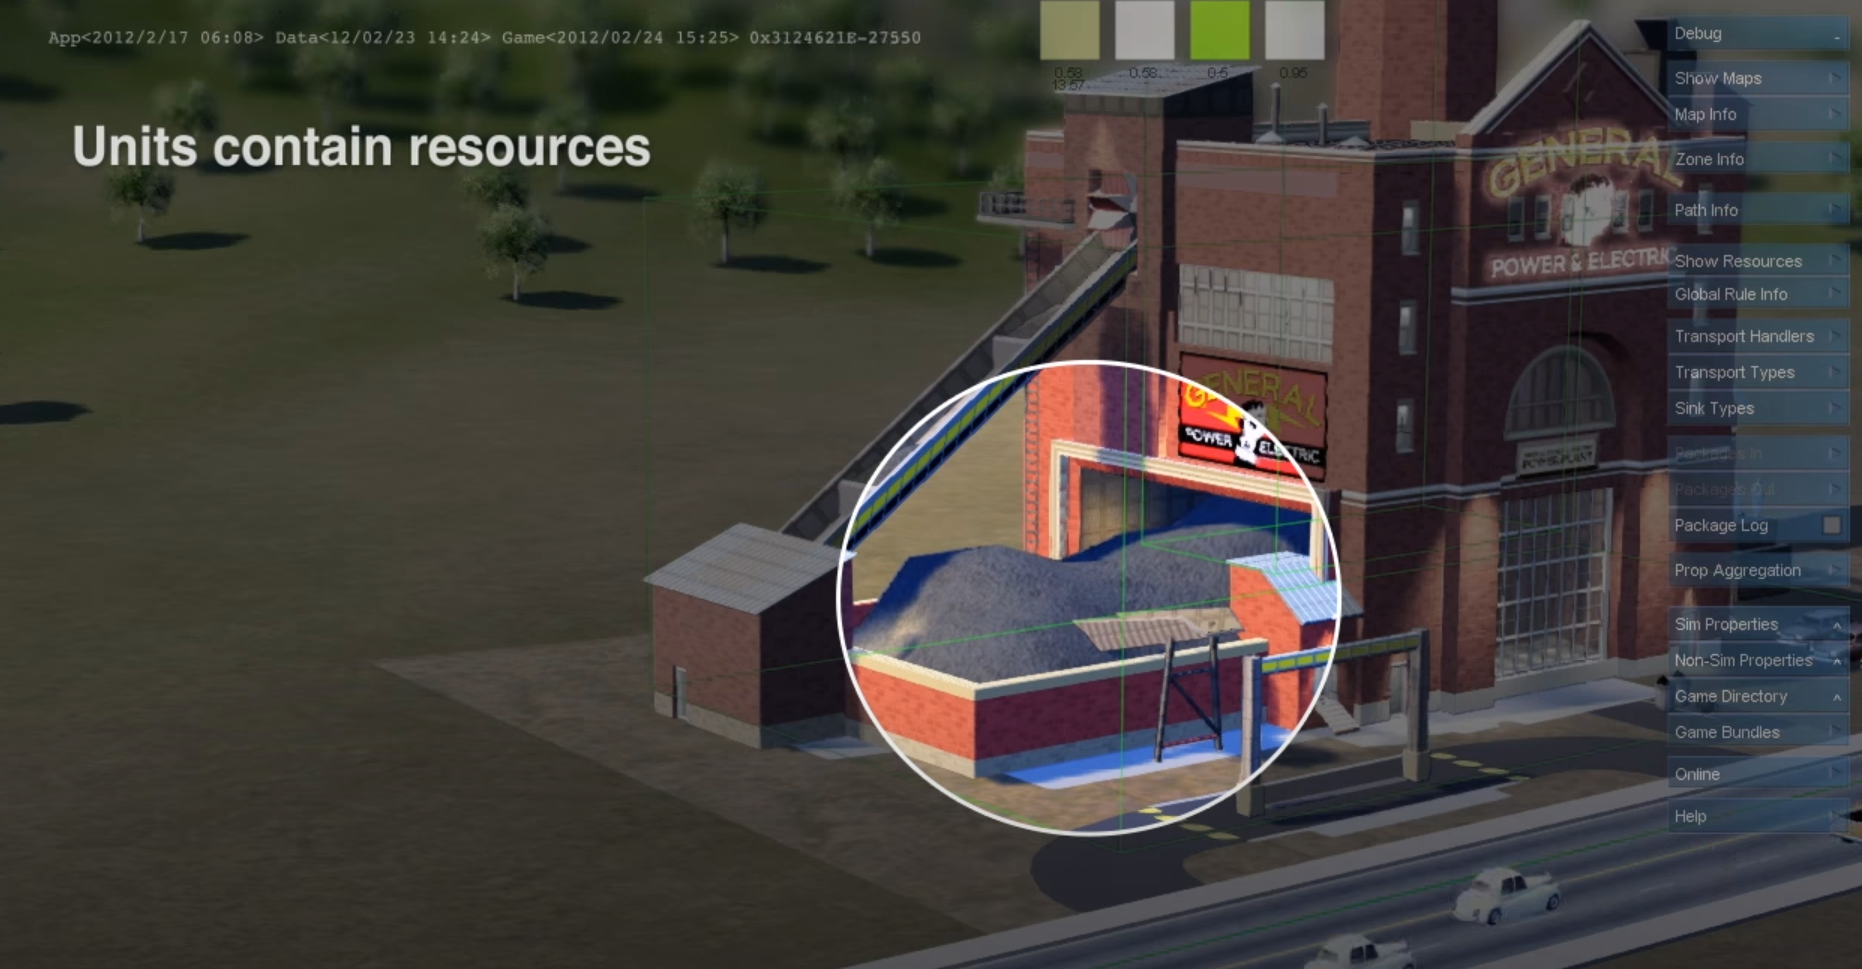
\includegraphics[width=0.7\textwidth]{gfx/resource}  	  	 	
	\caption{Power Station.\\ http://www.andrewwillmott.com/talks/inside-glassbox}
	\label{fig:example5_1}
\end{figure}

Core power unit simulates, contains resources as core and workers. When simulated, it runs simulation rules that use up cores to create power and air pollution(rules trigger effects). The facts of the animation are tied directly with the simulation rules, so what you see is what the simulation is doing. Drop additional units on the building like gerages to extend the area and functionality of the buildings.

\subsection{Maps}

Maps represent the consumable resources in an environment: coal, oil, forests, but also air pollution, land values, desirability, etc. For example, a map might have oil in the ground that is pumped out into its own local garbage can.

Maps defined the distribution of resources throughout the environment. Forest water and pollution are all represented in this map. The terrain is built up by this map as well. The terrain is driven by resources, Which contains rock core and soil.

\begin{figure}[htb]
	\centering
	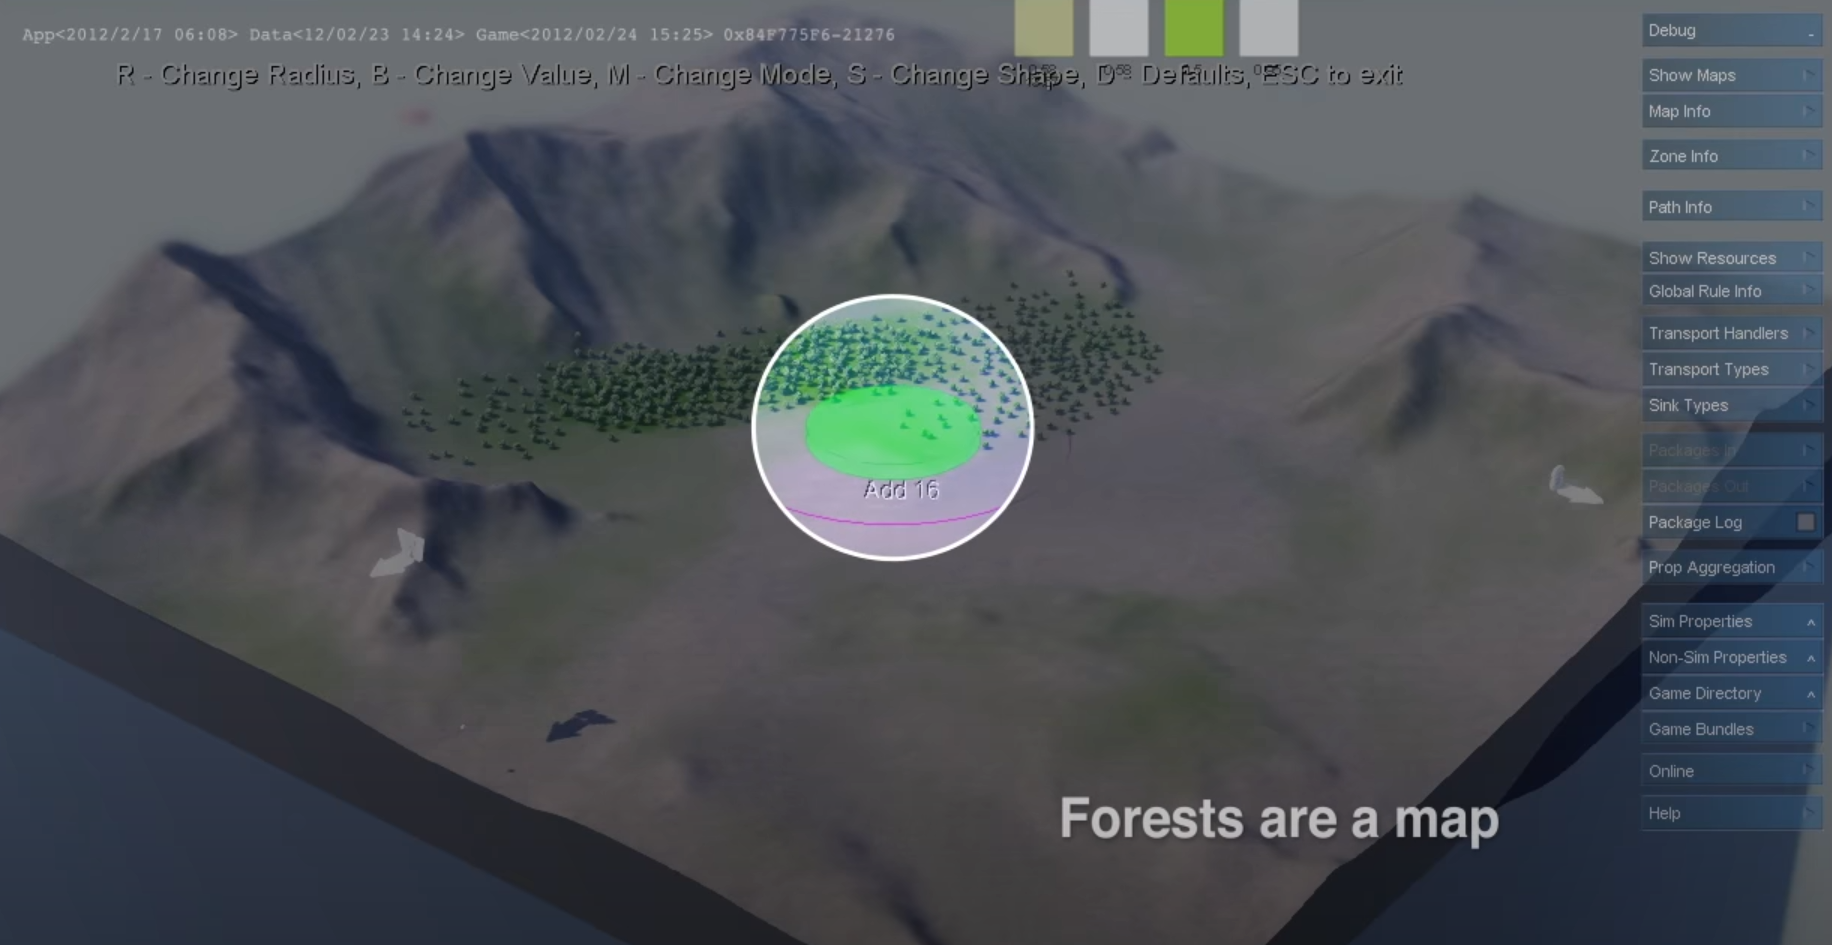
\includegraphics[width=0.7\textwidth]{gfx/Maps}  	  	 	
	\caption{Forest Map.\\ http://www.andrewwillmott.com/talks/inside-glassbox}
	\label{fig:example5_2}
\end{figure}

\subsection{Other}

There are also other aspects describe the behaviour of charactristics in the game. The collaboration of different globals can make the whole city work. global is represented in the game as agents, path and zones. 

Agents are simulation entities, which carry resources from one unit to another. The most common types of Agents are pedestrian and vehicles, which travelling around through the player defined path. The simulators are designed to support tens of thousands of Agents. Agents trigger the simulation rules when they arrive their destinations. But no rules runs during transit. Agents can also carry other types of resources throughout the city. They can drop off a portion of a power a water at each building and then the resend. Water taken from the water map is repackaged into Agents and long pipes. A destination is given to each agent, which decides whether they go to work or home, Jobs are determined by destionation as well. For instance, firemen may go into a fire.

Paths are made up by connected segments, which set up by points. A group of paths describe path sets. Path sets are fully 3D in the engine, and rich of operations. Not only roads are included in paths, but also power lines, water pipes and flight paths.

Zones are well-defined area described along a path. Zones run the rules to create, upgrade and destroy units. In this case, a residential construction sites. Agents such as construction moving vans deliver construction trials and new citizens.

\begin{figure}[htb]
	\centering	
	\subcaptionbox{Agent %
		\label{fig:example5_3}}%
	[.48\linewidth]{
		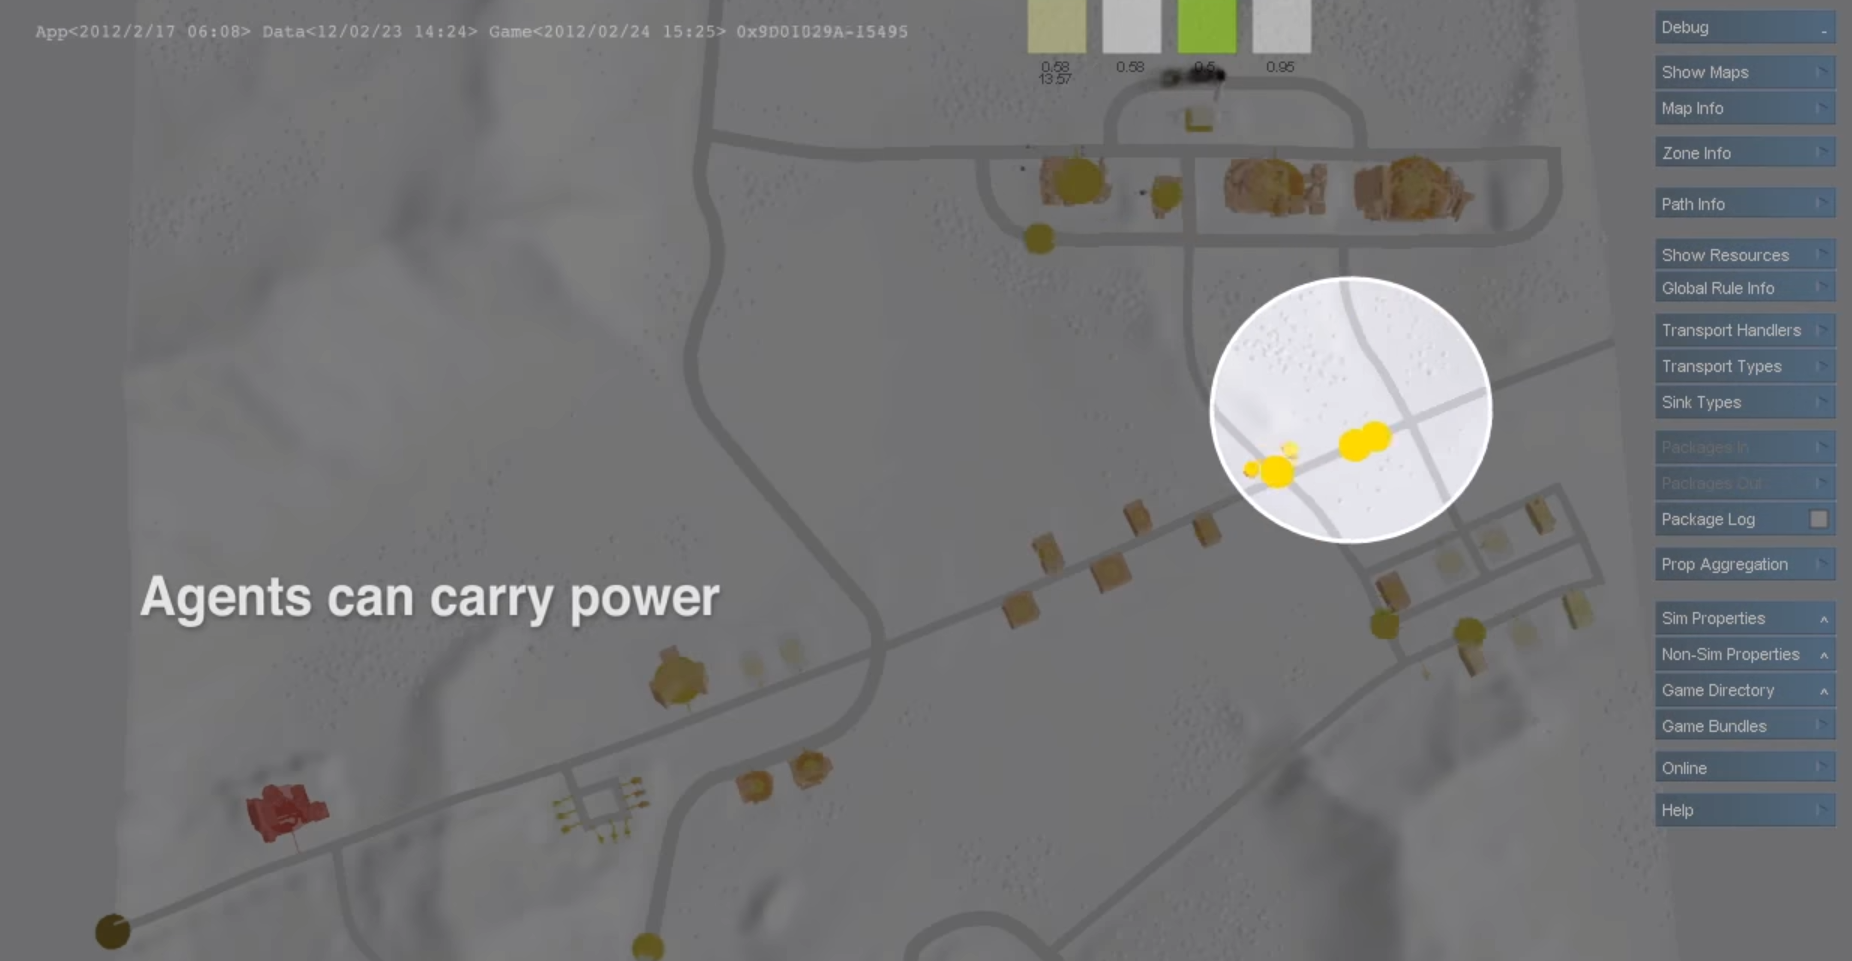
\includegraphics[width=0.45\textwidth]{gfx/other_1} 	
	}  	
	~
	\subcaptionbox{Path and Zone  %
		\label{fig:example5_4}}
	[.48\linewidth]{
		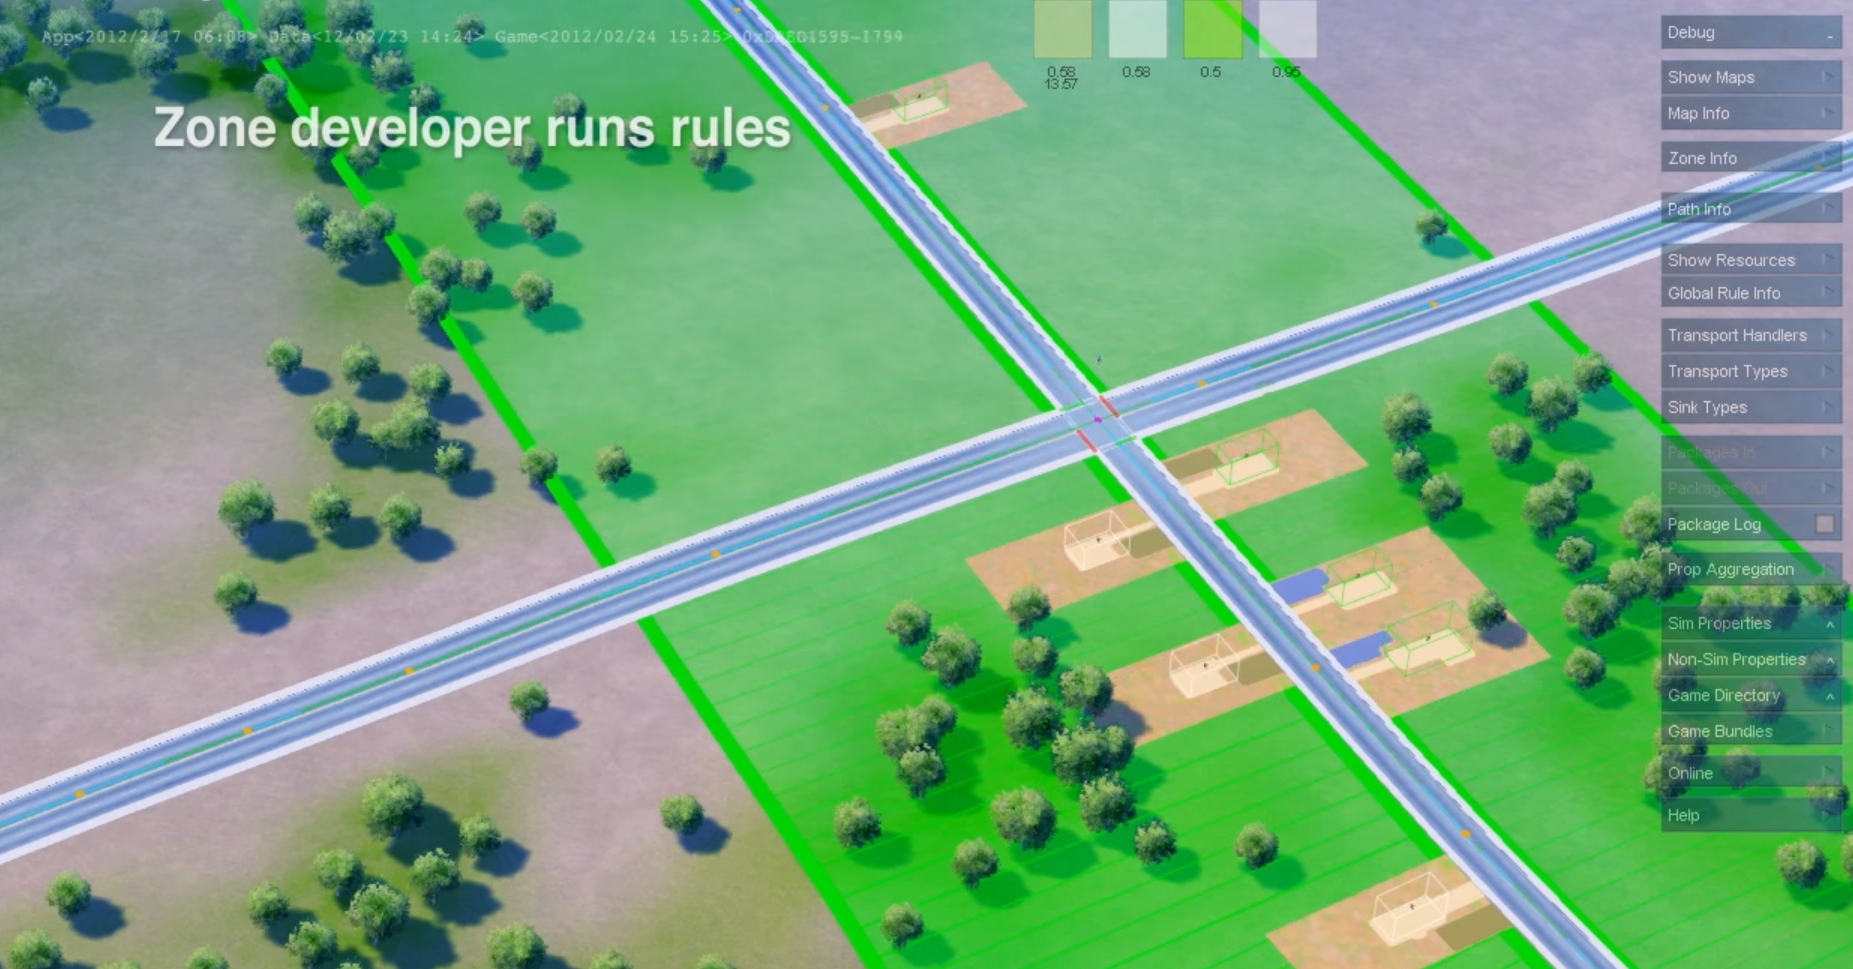
\includegraphics[width=0.45\textwidth]{gfx/other_2}  	
	}	  
	
	\caption{Agent Paths and Zones in GlassBox.\\ http://www.andrewwillmott.com/talks/inside-glassbox}
	\label{fig:ex_5}
\end{figure}



\subsection{Example: Water System}

Figure 3.4 shows an example of how GlassBox simulate the water system of a city. The first thing need to be considered is the water map around the city. The green area is wet and brown is dry area can be clearly seen. Based on the water map, a city can be clearly planned. 

\begin{figure}[htb]
	\centering	
	\subcaptionbox{Water Map with Buildings %
		\label{fig:example5_3}}%
	[.48\linewidth]{
		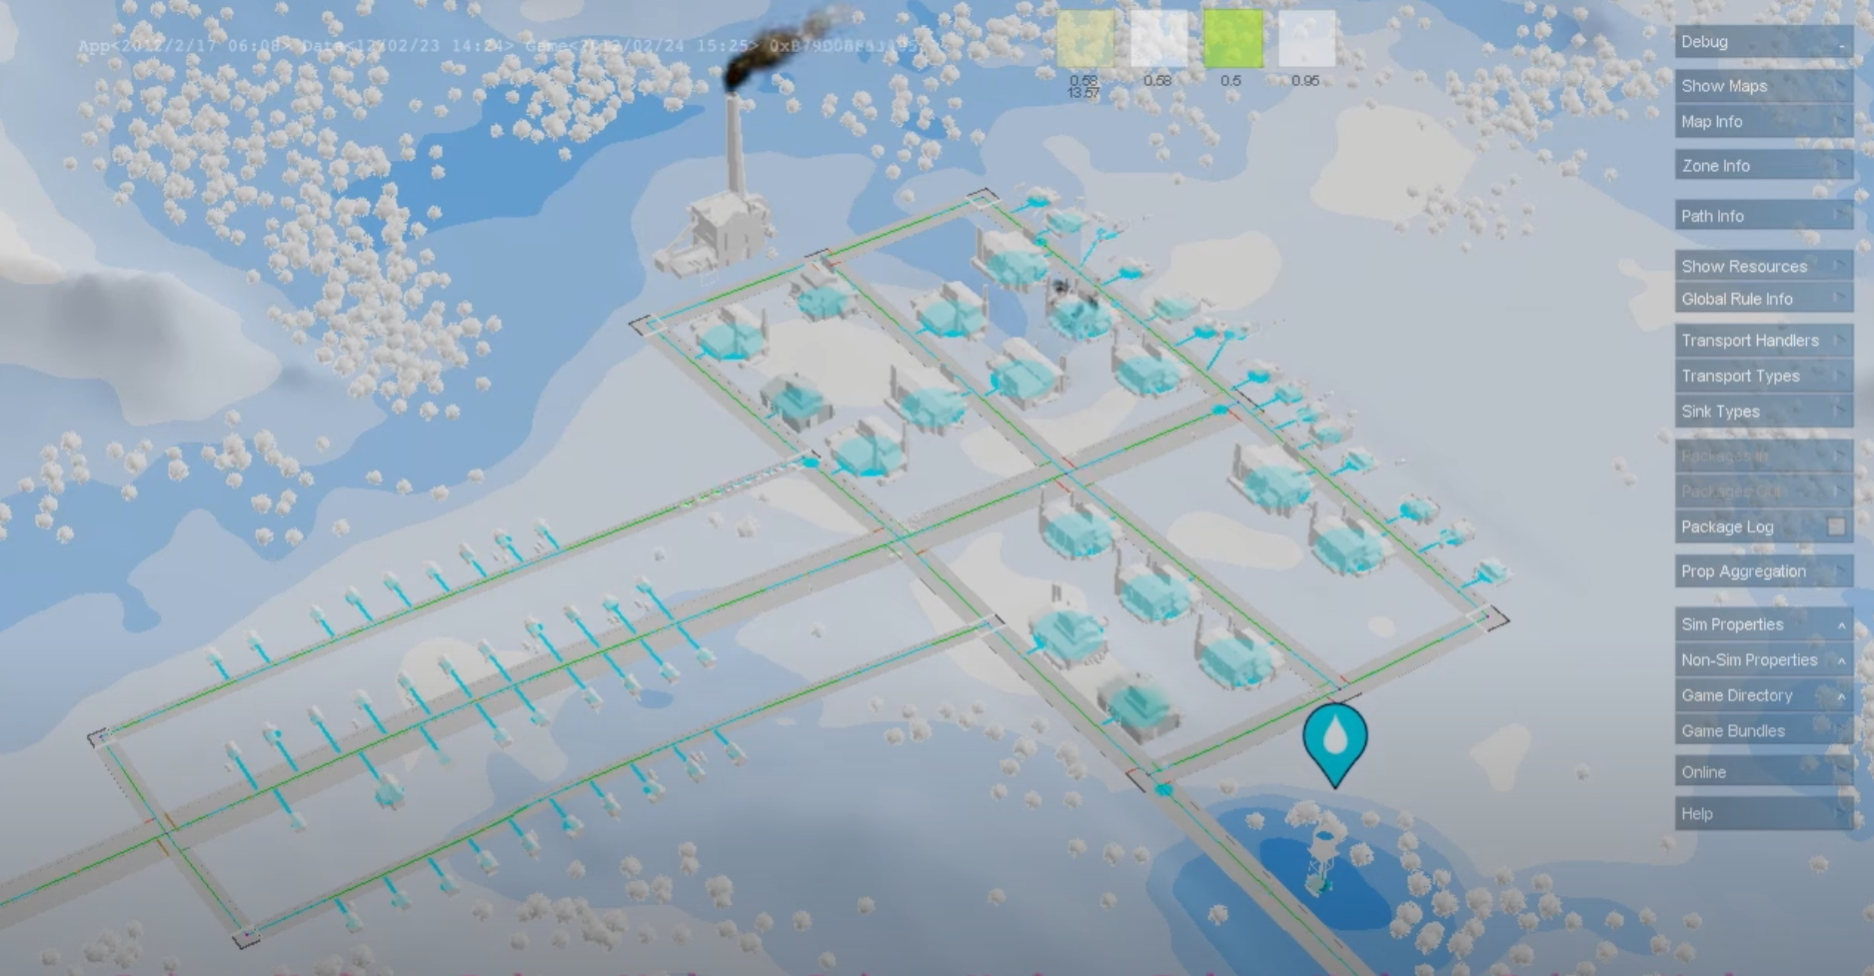
\includegraphics[width=0.45\textwidth]{gfx/water_1} 	
	}  	
	~
	\subcaptionbox{Water Map with Forest  %
		\label{fig:example5_4}}
	[.48\linewidth]{
		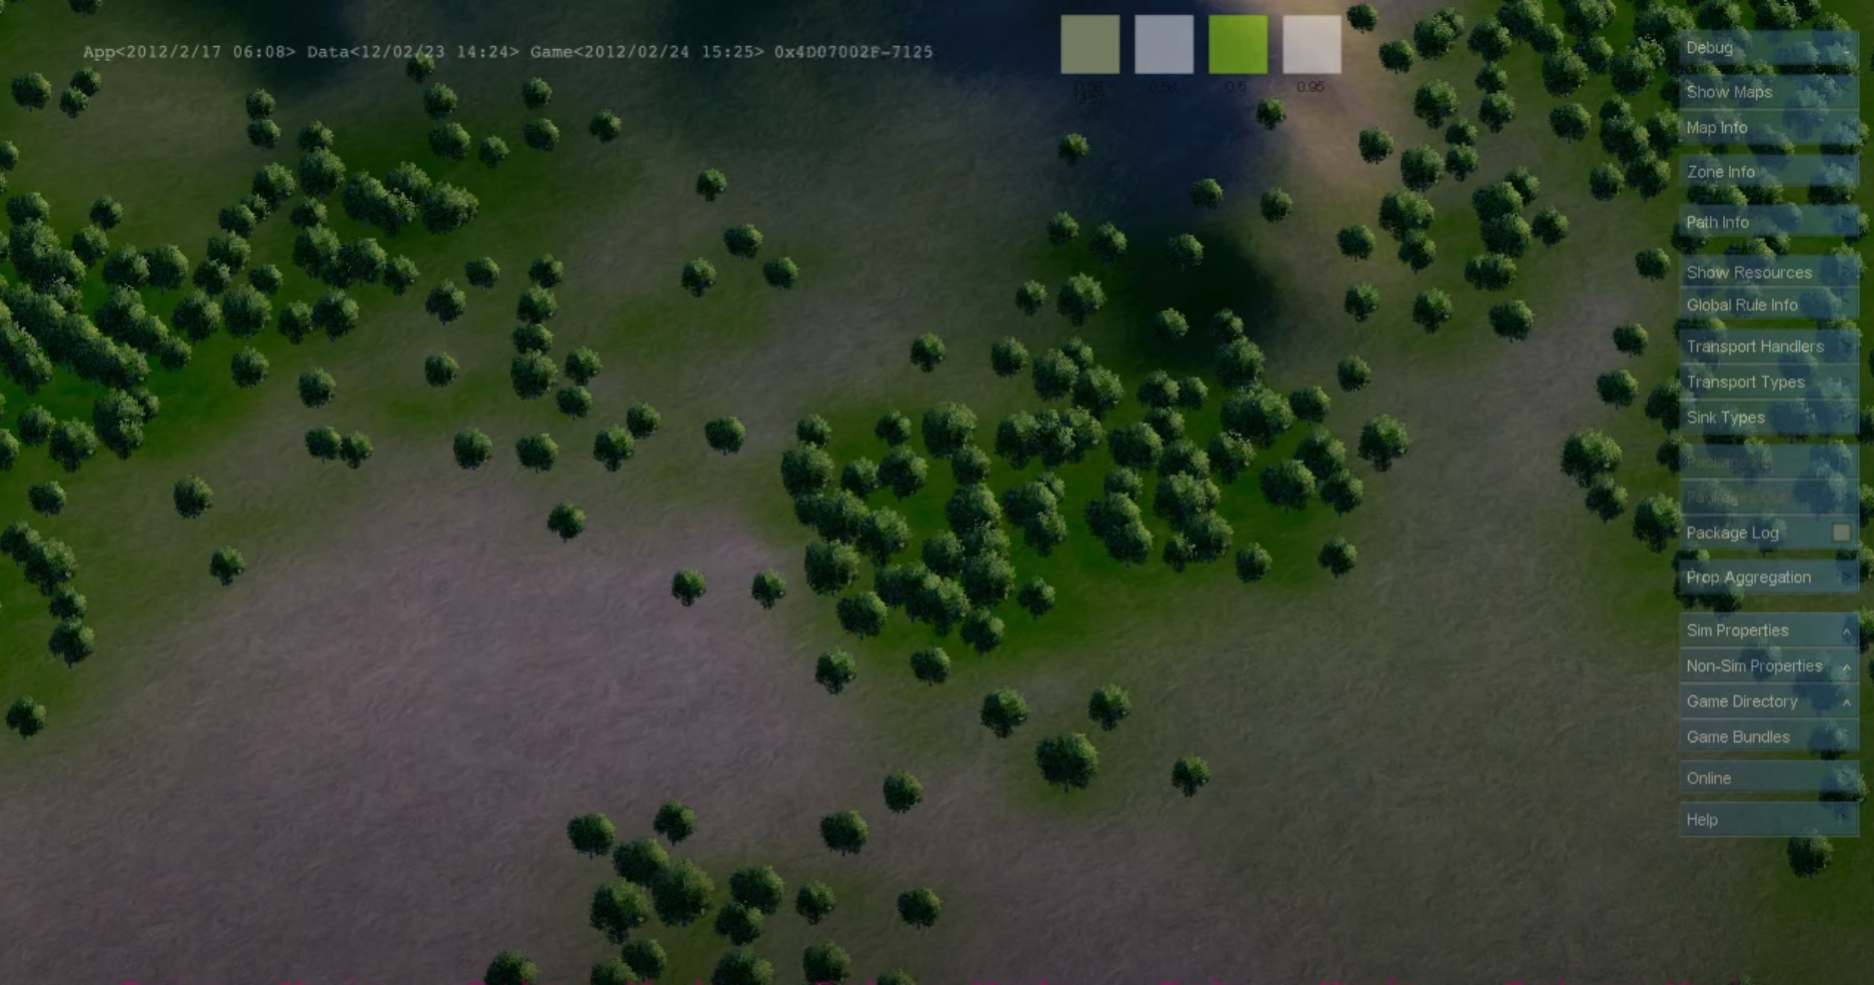
\includegraphics[width=0.45\textwidth]{gfx/water_2}  	
	}	  
	
	\caption{Water Maps in GlassBox.\\ http://www.andrewwillmott.com/talks/inside-glassbox}
	\label{fig:ex_5}
\end{figure}

Some units are avaliable for running a water system. Water tower in Figure 3.5 is the simulation unit that runs the rules arrive your city with water. With pumping animation, it substracting the ground water from the water table map. As it pumps, the water that is pulled to the ground, repackaged and sent out as simulation agents that travel down to the pipes, then transferred to the water consuming buildings. The buildings periodically use the water based on the rules, which will be talked in next section, and produce some products with citizens.

\begin{figure}[htb]
	\centering	
	\subcaptionbox{Water Tower %
		\label{fig:example5_3}}%
	[.48\linewidth]{
		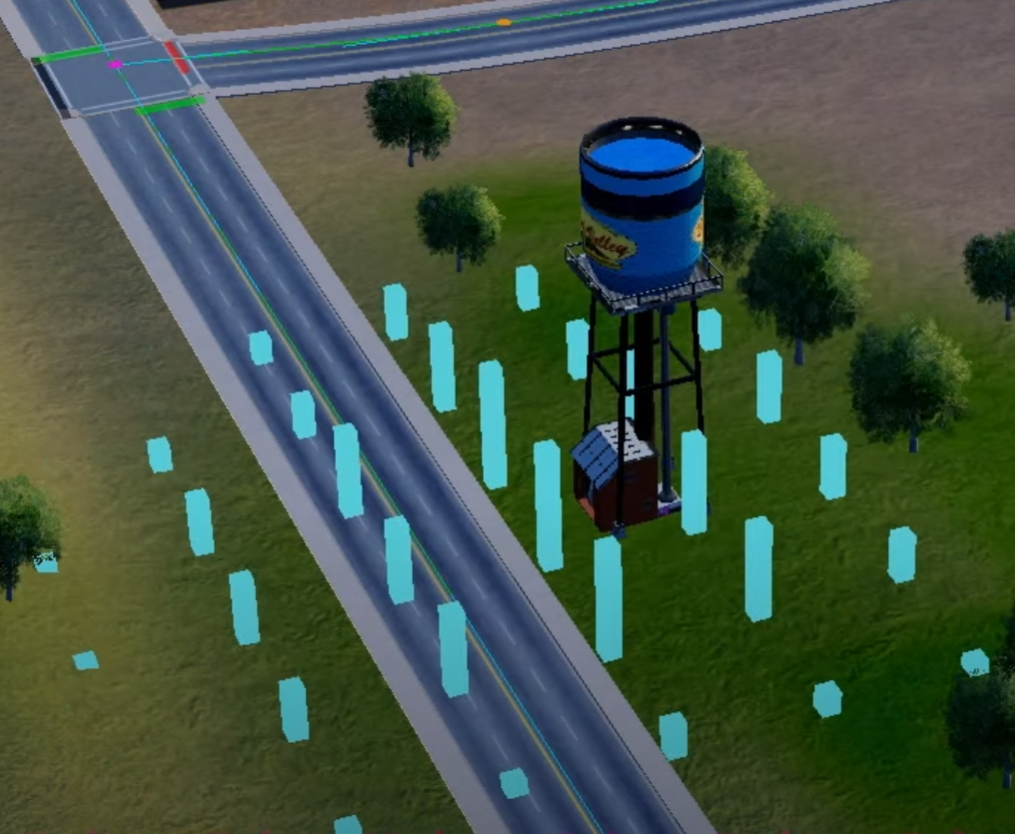
\includegraphics[height=0.25\textwidth]{gfx/water_3} 	
	}  	
	~
	\subcaptionbox{Water Consuming Buildings  %
		\label{fig:example5_4}}
	[.48\linewidth]{
		\includegraphics[width=0.45\textwidth]{gfx/water_4}  	
	}	  
	
	\caption{Water System in GlassBox.\\ http://www.andrewwillmott.com/talks/inside-glassbox}
	\label{fig:ex_5}
\end{figure}

Meanwhile, industrial area will produce lots of ground pollution, and ground pollution influence the water power. Now when the water tower pump water to the ground, also picking some ground pollution, sending out with agents. When this water consumed it causes sickness. Sick citizens can not work so it makes the economic decline in your city.

\begin{figure}[htb]
	\centering	
	\subcaptionbox{Sickness of Citizens %
		\label{fig:example5_3}}%
	[.48\linewidth]{
		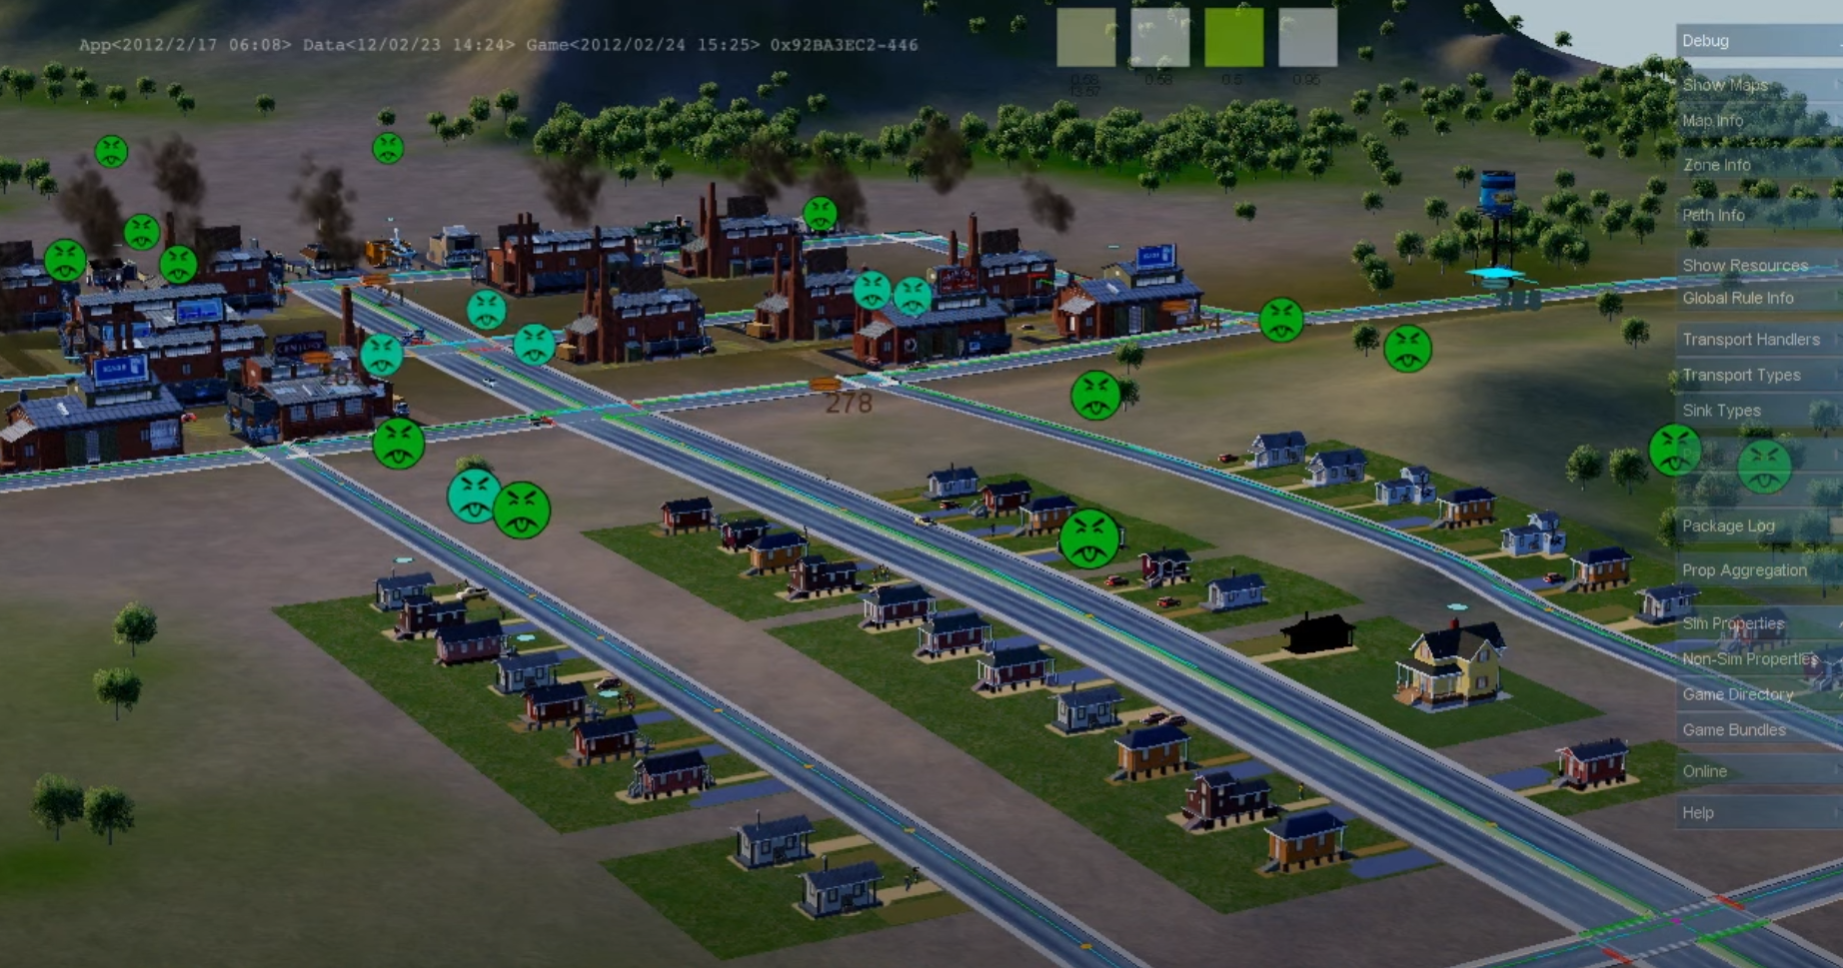
\includegraphics[width=0.45\textwidth]{gfx/water_5} 	
	}  	
	~
	\subcaptionbox{Water Pollution  %
		\label{fig:example5_4}}
	[.48\linewidth]{
		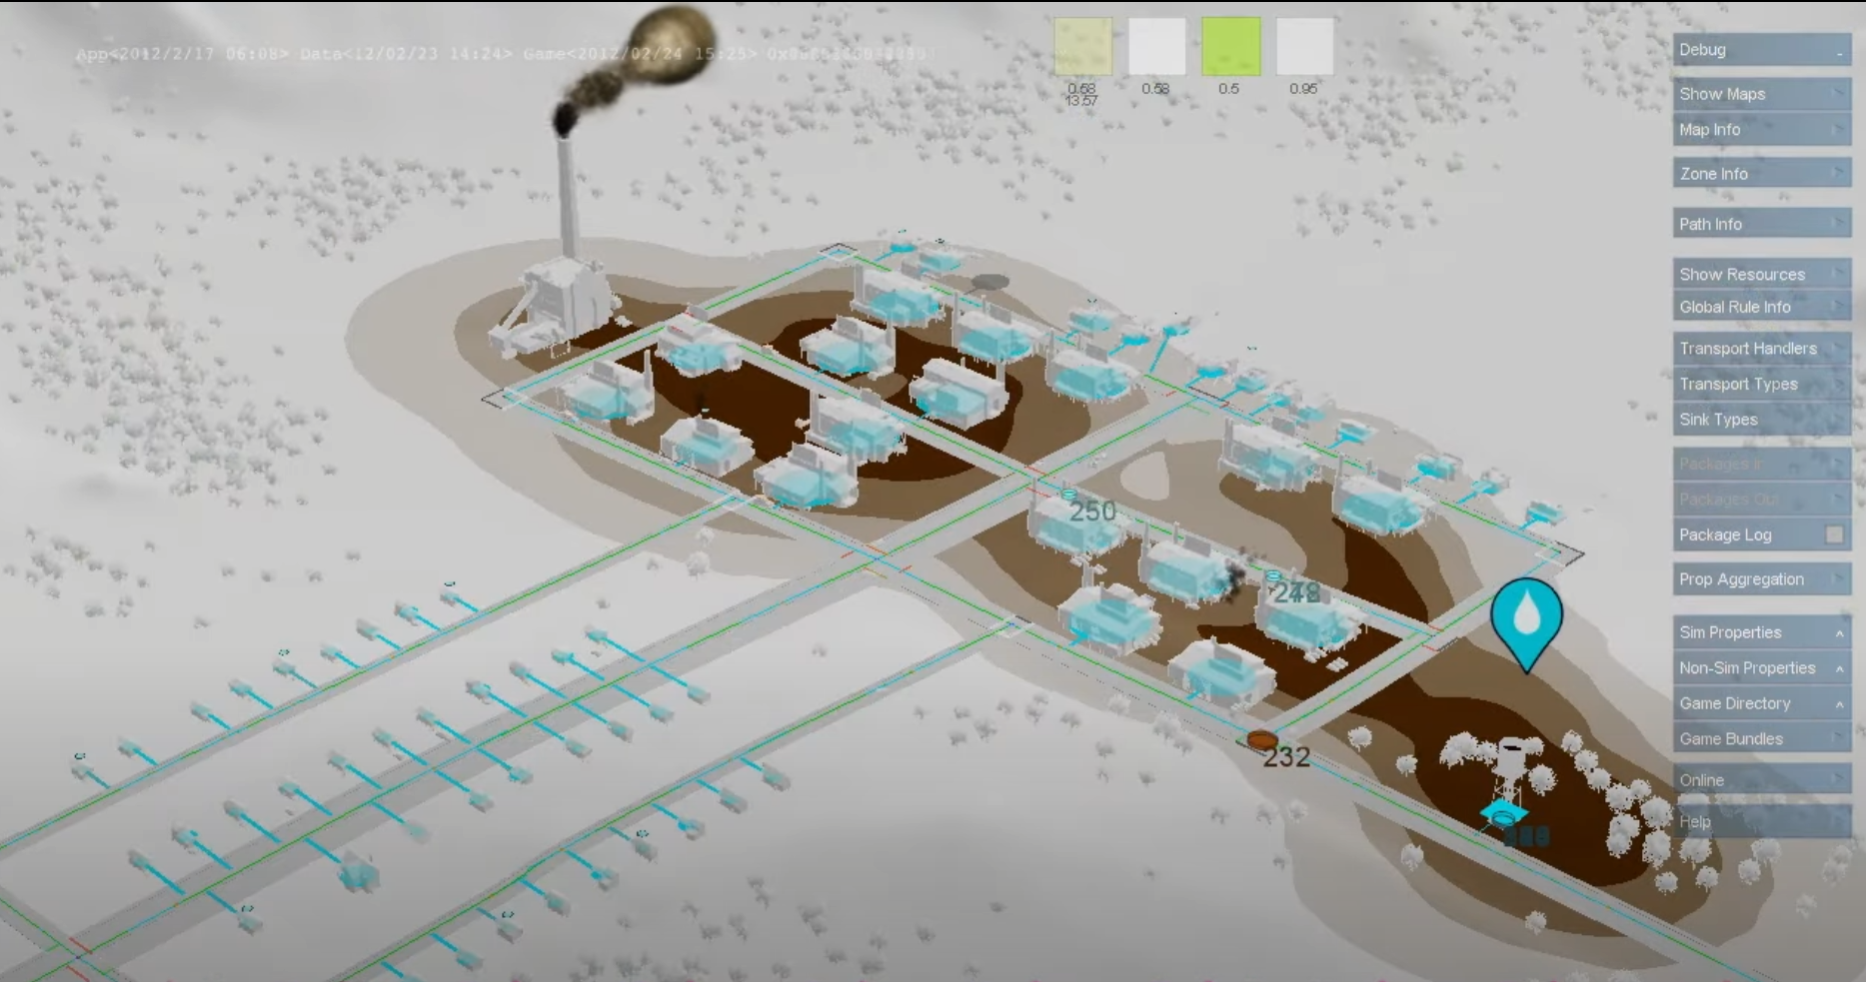
\includegraphics[width=0.45\textwidth]{gfx/water_6}  	
	}	  
	
	\caption{Water Problems.\\ http://www.andrewwillmott.com/talks/inside-glassbox}
	\label{fig:ex_5}
\end{figure}

\subsection{Game Logic}

Game logic is the rule of simulation in GlassBox, which garanteens the operation of the city. 

\section{Summary}

%*****************************************
\chapter{Application}

\section{Use Case}

\subsection{Taxonomy Use Cases}

\section{Digital Twins}

\section{Smart City}



%*****************************************
\chapter{Discussion}


\chapter{Conclusion}
